\chapter{\ac{ser} Development}
\label{chapter:strat}

\section{Datasets}

In this section, we present a detailed account of the datasets employed in the development and evaluation of our \ac{ser} system.

The first dataset was utilized to investigate and select the most optimal features and evaluate the performance of classification models and effective classification strategies.

\subsection{\ac{iemo}}

The \ac{iemo} database \cite{Busso2008}, created in \citeyear{Busso2008}, is an acted and elicited multimodal and multi-speaker database. It consists of 12 hours of audiovisual data, including video, speech, motion capture of face, and text transcriptions.

Sessions were manually segmented into utterances, spoken by 10 (5 female and 5 male) professional actors in fluent English. Each utterance was annotated by at least 3 human annotators in 9 categorical attributes, and, in addition, it was annotated with 3-dimensional attributes using the \ac{vad} emotion model. Similar to the development dataset, this data was collected using emotion elicitation techniques such as improvisations and scripts. Figure \ref{fig:bar_plots_distribution} from the research  \cite{Busso2008}, demonstrates a similar amount of annotated labels on scripted and spontaneous sessions on this dataset.

\begin{figure}[H]
	\centering
	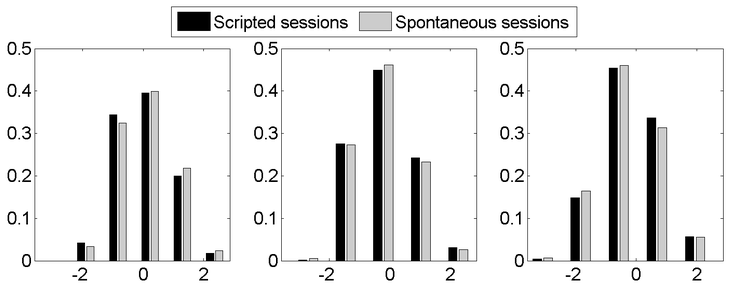
\includegraphics[width=.8\linewidth]{figs/4_1_traditional/scripted_spont_distribution.png}
	\caption{Distribution of the emotional content of the IEMOCAP corpus in terms of (a) valence, (b) activation, and (c) dominance. The results are separately displayed for scripted (black) and spontaneous (gray) sessions.}
	\label{fig:bar_plots_distribution}
\end{figure}

Most researchers when using this dataset perform 4 class emotion recognition, and also, consider the emotion excitement as happiness, due to their similarities and to even out the distribution of files per emotion. We decided to use the same data, as shown in Table \ref{tab:all_datasets}, ending up with a total of 5531 audio files recorded with a sample rate of 16000 Hertz.

Overall, \ac{iemo} is a well-suited resource for our study, as the multimodal data, annotated using both discrete and dimensional models, allows us to perform a wide range of operations. Several Researchers have also noted the high quality of this dataset, being frequently used in the literature for evaluating emotion recognition models. This enables us to compare our developed models effectively, which is why we utilized it as a training and testing dataset for our \ac{ser} models and to explore classification strategies and their biases.

\subsection{Testing Datasets}

To evaluate the generalization ability of our final models trained on the IEMOCAP dataset, we tested them on three additional emotion datasets: eNTERFACE’05, CREMA-D, and EMO-DB. The inclusion of these datasets allows us to assess the efficacy and applicability of our proposed \ac{ser} system across diverse contexts and conditions. For all three testing datasets, we only used the set of 4 emotions present in the \ac{iemo}.

The eNTERFACE’05 emotion database \cite{Martin2006} was designed and collected during the eNTERFACE’05 workshop. This dataset contains discrete annotated emotions, where each subject was asked to listen to six successive short stories, each eliciting a particular emotion. The dataset contains audio and visual data from 42 subjects, coming from 14 different nationalities. Among the subjects, a percentage of 35 are men, while the remaining 7 are women, and, all the experiments were driven in English. The diversity of accents present in the dataset and its authenticity (due to the data being elicited), make it a suitable choice for testing the models' performance with different factors than the \ac{iemo}. The number of used files per emotion is presented in Table \ref{tab:all_datasets}.

The EMO-DB database is an acted German emotional database created by the Institute of Communication Science, Technical University, Berlin, Germany. Ten professional speakers (gender-balanced) participated in the data recording. This dataset is composed of a total of 339 audio files annotated with the four emotions used in the \ac{iemo}, shown in table \ref{tab:all_datasets}, making it a small-sized dataset. However, it allows us to test more directly the models' limitations, mostly the language bias since it provides files in a different spoken language than the training dataset. 

The CREMA-D dataset includes clips from 91 actors spoken in English. These clips are from 48 male and 43 female actors between the ages of 20 and 74 coming from a variety of races and ethnicities (African American, Asian, Caucasian, Hispanic, and Unspecified). It provides a variety of data which is ideal to test a model's generalization ability across new datasets. The sentences were presented using one of six different emotions, but as mentioned before, we selected only the emotions present in the \ac{iemo}, resulting in 4898 audio files \ref{tab:all_datasets}. 



\begin{table}[H]
	\centering
	\caption{Number of audio files per emotion from the described datasets.}
	\label{tab:all_datasets}
	\begin{tabular}{lrrrr}
		\toprule
		& \multicolumn{4}{c}{Number of Files} \\
		\cmidrule{2-5}
		Emotion     &   \ac{iemo} & eNTERFACE'05 & EMO-DB & CREMA-D \\
		\midrule
		Anger   	&         1103 &  210 & 127 & 1271 \\
		Happiness   &         1636 &  210 &  71 & 1271 \\
		Neutral		&         1708 &    0 &  79 & 1087 \\
		Sadness     &         1084 &  210 &  62 & 1269 \\
		\bottomrule
	\end{tabular}
\end{table}


